\documentclass[12pt,a4paper]{report} %Formato y formas principales
\usepackage[spanish]{babel} %Establecer idioma
\usepackage{graphicx} %Para añadir imágenes
\usepackage{fancyhdr} %Para establecer mi propio encabezado y pie de página
\usepackage[left=3cm,right=3cm,top=2.5cm,bottom=2.5cm,headsep=1cm]{geometry} % Mis márgenes
%\setlength{\headheight}{14.0pt} %Ajusta el tamaño del encabezado
%\linespread{1.5} % Espaciado de 1.5 (1 es el espaciado estándar)
\setlength{\parindent}{0pt} %Ajusta la sangría a 0 para que no haya
\usepackage{amsmath} %Para ecuaciones\usepackage{amsmath}
\usepackage{multicol}
%\usepackage{refcheck} %Para que aparezca el nombre que le doy a la referencia
\usepackage{comment} %Para comentar varias lineas
\usepackage{lipsum} %Para hacer textos de ejemplo para pruebas
\usepackage{bm} % Agrega esta línea en el preámbulo del documento

\usepackage{caption} %Para crear mi formato "boldformat" que pone lo primero en negrita
\DeclareCaptionFormat{boldformat}{\textbf{#1} #2 #3}
\captionsetup[figure]{format=boldformat} %Le asigno el formato al de las figuras

\usepackage{hyperref} %Para que haya hipervínculos
\hypersetup{
	colorlinks=true, %Para que los hipervínculos sean de color y no con caja roja
	linkcolor=blue,
	urlcolor=black,
	citecolor=blue,
}

\makeatletter %Mi propio comando para establecer las referencias de figuras y ecuaciones
\newcommand{\fref}[1]{\hyperref[#1]{\textcolor{blue}{\textit{Fig.~\ref*{#1}}}}}
\newcommand{\eref}[1]{\hyperref[#1]{\textcolor{blue}{\textit{(\ref*{#1})}}}}
\makeatother

\usepackage{makeidx} %Para hacer el indice
\makeindex
\usepackage{tocloft} %Para configurar el índice
\renewcommand{\cftchapleader}{\cftdotfill{\cftdotsep}} %Línea puntos índice
\setlength{\cftbeforetoctitleskip}{-1cm} % Ajusta el margen superior del índice

\usepackage[T1]{fontenc} %Para cambiar la letra y el tamaño
\usepackage[scaled]{uarial}
\renewcommand*\familydefault{\sfdefault}


\usepackage{titlesec} %Para cambiar mi formato de chapter
\titleformat{\chapter}[display]
{\normalfont\huge\bfseries}{\chaptertitlename\ \thechapter}{20pt}{\LARGE}
\titlespacing*{\chapter}{0pt}{-1.5cm}{40pt}

\pagestyle{fancy}
\fancyhf{}
\fancyhead[L]{\fontsize{12}{14}\selectfont\leftmark}  % Número de página a 
\fancyhead[R]{\fontsize{12}{14}\selectfont\thepage}  % Número de página 
\fancyfoot[R]{\fontsize{12}{14}\selectfont Sevilla, Julio de 2023}  



\begin{document}
	
	\begin{titlepage}
		\centering
		\hspace*{-1.5cm}\begin{tabular}{@{}l@{}}
			
\includegraphics[width=3cm]{b.png} % Logo 1 (esquina superior izquierda)
		\end{tabular}
		\hfill
		\begin{tabular}{c}
			\LARGE\textbf{Universidad de Sevilla} \\ [0.5cm] % Nombre de la universidad
			\LARGE\textbf{Escuela Politécnica Superior} % Otra frase dentro de la misma caja
		\end{tabular}%
		\hfill
		\begin{tabular}{@{}r@{}}
			
\includegraphics[width=3cm]{a.png} % Logo 2 (esquina superior derecha)
		\end{tabular}\hspace*{-1.5cm}
		
		\vspace{1.5cm}
		
		\begin{center}
			\Large\textmd{Trabajo Fin de Grado} \\ [0.2cm] % Título 
			\Large\textmd{Ingeniería Electrónica Industrial}
		\end{center}
		
		\vspace{2cm}
		
		\begin{center}
			\LARGE\textsl{La caracterización integral de las semiaplicaciones de Poincaré y su aplicación a circuitos electrónicos: El Memristor}
		\end{center}
		
		\vspace{7cm}
		
		\raggedright
		\large\textbf{Autor:} Sergio R. Durán Martín \\ [0.5cm]
		\large\textbf{Tutor:} Dr. Victoriano Carmona Centeno \\ [0.5cm]
		\large\textbf{Departamento:} Matemática Aplicada II
	\end{titlepage}
	
	\clearpage
	\null
	\thispagestyle{empty}
	\newpage

\begin{center}
	\LARGE\textbf{Resumen}
\end{center}
\begin{minipage}{\textwidth}
	\lipsum[1]
	
	\vspace{0.5cm}
	\noindent \textbf{Palabras clave:} robótica educativa, robot modular, STM32, FreeRTOS, interfaz gráfica, impresión 3D.
\end{minipage}

\vspace{1cm}

\begin{center}
	\LARGE\textbf{Abstract}
\end{center}
\begin{minipage}{\textwidth}
	\lipsum[2]
	
	\vspace{0.5cm}
	\noindent \textbf{Keywords:} educational robotics, modular robot, STM32, FreeRTOS, graphic interface, 3D printing.
\end{minipage}
\newpage
	
\tableofcontents
	\chapter{Introducción}
	Contenido del capítulo de introducción. Contenido del capítulo 1.
	
	\chapter{Descripción del Circuito}
	El circuito que se ha estudiado es un oscilador con resistencia negativa al que se le ha añadido un componente muy interesante y que está siendo muy estudiado en estos últimos tiempos, el memristor, ver \fref{fig:-RLCM}.
	
	\begin{figure}[h]
		\centering
		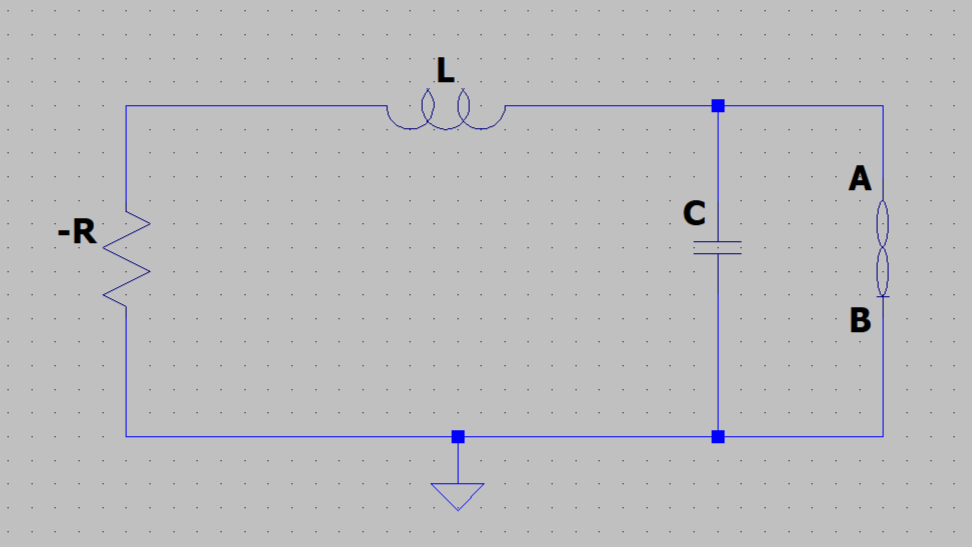
\includegraphics[width=0.7\textwidth]{-RLCM.png}
		\caption{Oscilador RLC con R negativa y Memristor}
		\label{fig:-RLCM}
	\end{figure}
	
	Como se puede ver no existe una fuente de señal en el circuito y esto se debe a que el análisis hecho busca encontrar una oscilación periódica tan solo proporcionando condiciones iniciales a la bobina y el condensador, esto gracias al comportamiento de la resistencia negativa y del memristor los cuales se especifican mas adelante.\\[0.5cm]
	La forma de imponer las condiciones iniciales serían las clásicas, usando fuentes de intensidad en serie y tensión en paralelo con interruptores que se abren en $t\,=\,0(s)$ para la bobina y el condensador respectivamente. Esta parte no se va a detallar más en profundidad puesto que en este trabajo no hay implementación real del circuito, los motivos se detallan en el CAPITULO X.
	\newpage
	\section{Resistencia negativa}
	Uno de los componentes del circuito es la resistencia negativa la cual se puede construir con lo que se llama un \emph{Convertidor de Impedancia Negativa (NIC)}. Un NIC es un circuito activo, es decir, en lugar de disipar energía como una resistencia convencional, puede proporcionar energía a un circuito, ver \fref{fig:NIC}. En términos prácticos, un NIC puede ser utilizado para compensar la resistencia de carga de un sistema, mejorar la eficiencia de la transferencia de energía o realizar otras funciones específicas en circuitos eléctricos o electrónicos. En los circuitos osciladores, el NIC desempeña un papel importante en el mantenimiento, estabilización, frecuencia y calidad de la oscilación.
	 
	\begin{figure}[h]
		\centering
		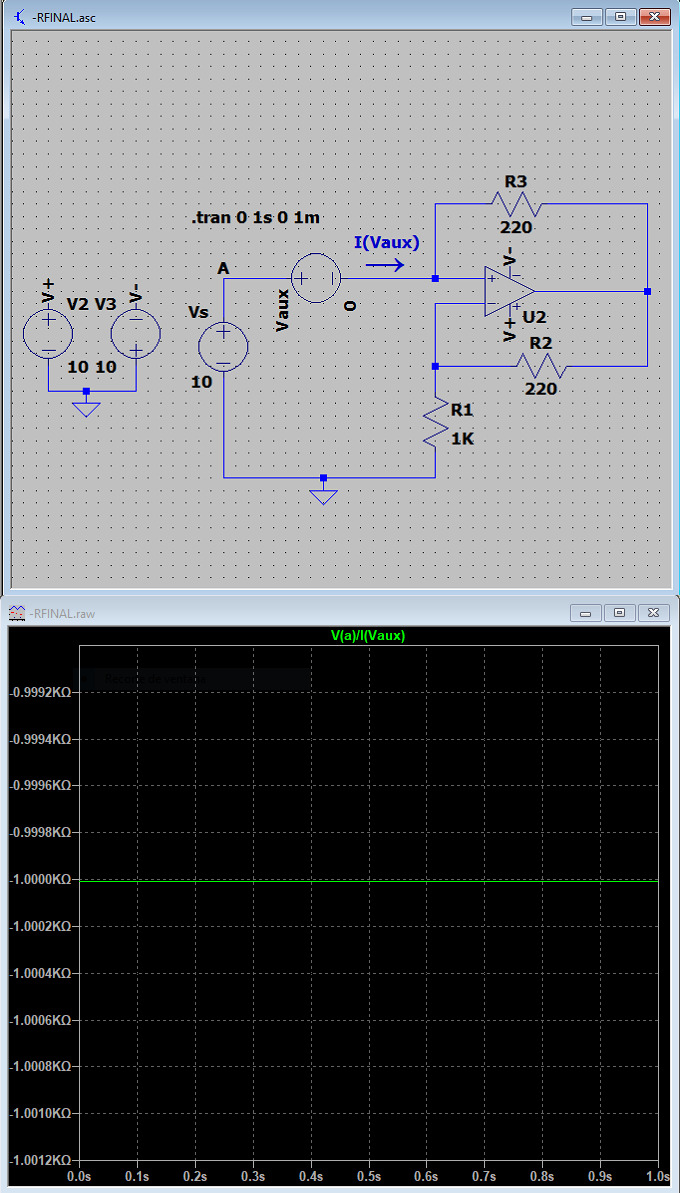
\includegraphics[width=0.65\textwidth]{NIC_B.jpg}
		\caption{Convertidor de Impedancia Negativa de -1000 Ohmios}
		\label{fig:NIC}
	\end{figure}
	
	\newpage
	
	Una de las maneras de realizarlo es usando un amplificador operacional y 3 resistencias en la configuración que se ve en la \fref{fig:NIC} de esta manera si elegimos $R_2=R_3$ la resistencia $R_1$ es la que determinaría el valor de resistencia negativa, esta es la demostración:
	
	\begin{center}
	\begin{multicols}{2}
		\centering
		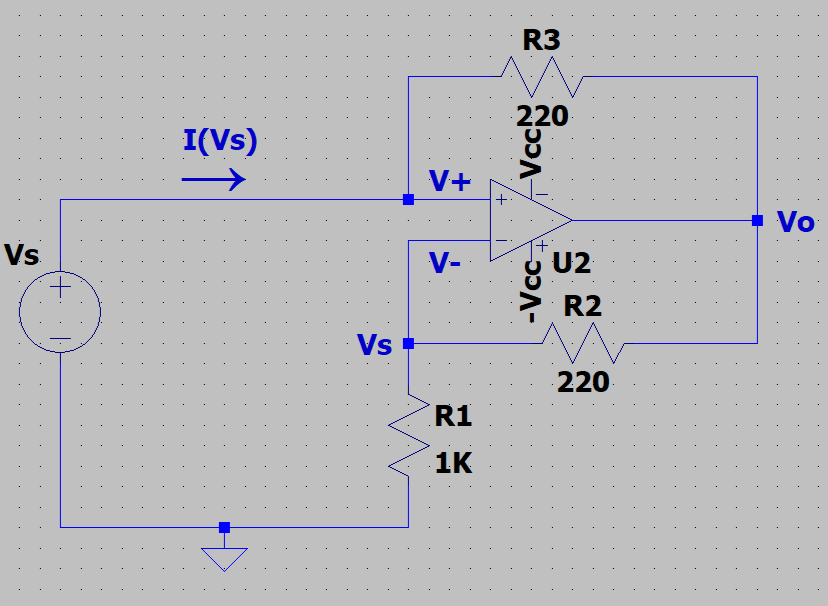
\includegraphics[width=\columnwidth]{demotracion_NIC.png}
		\captionof{figure}{Parámetros circuito NIC }
		\label{fig:Param_NIC}
	
		\columnbreak
		
		Consideraciones para el cálculo del circuito de la \fref{fig:Param_NIC} con Amplificadores Operacionales:\\
		\begin{equation}
			V_+\,=\,V_-
			\label{eq:NIC1}
		\end{equation}
		\begin{equation}
			I_+\,=\,I_-\,=\,0\,(A)
			\label{eq:NIC2}
		\end{equation}
	\end{multicols}
	\end{center}
	
	Teniendo en cuenta la ecuación \eref{eq:NIC1} se puede ver que la tensión $V_S$ cae sobre $R_1$ y se puede relacionar con $V_O$ mediante un divisor de tensión:
	
	\begin{equation}
		V_S\,=\,V_O\,\frac{R_1}{R_1 + R_2}\:\longrightarrow\:V_O\,=\,V_S\,\frac{R_1 + R_2}{R_1}
		\label{eq:NIC3}
	\end{equation}\smallskip
	
	Teniendo en cuenta la ecuación \eref{eq:NIC2} se puede ver que la intensidad $I(V_S)$ es la misma que pasa por la $R_3$, por ello se puede deducir:
	
	\begin{equation}
		I(V_S)\,=\,\frac{V_S - V_O}{R_3}
		\label{eq:NIC4}
	\end{equation}\smallskip
	
	Sustituyendo la ecuación \eref{eq:NIC3} en \eref{eq:NIC4} y trabajando la expresión se llega a:
	
	\begin{equation}
		I(V_S)\,=V_S\,\frac{-R_2}{R_1 \, R_3}
		\label{eq:NIC5}
	\end{equation}\smallskip
	
	Si dividimos $V_S$ entre $I(V_S)$ (ecuación \eref{eq:NIC5}) para obtener la impedancia de entrada:
	
	\begin{equation}
		\frac{V_S}{I(V_S)}\,=\,Z_{IN}\,=\,\frac{V_S}{V_S\,\frac{-R_2}{R_1 \, R_3}}\,=\,-R_1\,\frac{R_3}{R_2}
		\label{eq:NIC6}
	\end{equation}\smallskip
	
	Si elegimos $R_3\,=\,R_2$ en la ecuación \eref{eq:NIC6} obtenemos:
	
	\begin{equation}
		Z_{IN}\,=\,-R_1
		\label{eq:NIC7}
	\end{equation}\smallskip
	
	\newpage
	\section{Memristor}
	El componente más interesante de este circuito es el Memristor, teorizado por el científico Leon Chua en 1971 \cite{chuamissing1971}, este elemento trata de llenar el vacío que existía en las relaciones entre las cuatro variables básicas en teoría de circuitos: voltaje \textbf{\textit{v}}, intensidad \textbf{\textit{i}}, carga eléctrica \textbf{\textit{q}} y flujo magnético \textit{$\bm{\varphi}$}. En concreto el memristor relaciona la carga eléctrica con el flujo magnético de la siguiente manera \cite{chuaoscillator2008}:
	
	\begin{equation}
		\varphi\,=\,\varphi(q) \qquad q\,=\,q(\varphi)
		\label{eq:flujocarga}
	\end{equation}\smallskip
	
	Sabiendo la relacion del voltaje y la intensidad respecto a la carga y al flujo en el tiempo:

	\begin{equation}
		v(t)\,=\,\frac{d\varphi}{dt} \qquad i(t)\,=\,\frac{dq}{dt}
		\label{eq:dvdi}
	\end{equation}
			
	\begin{equation}
		\varphi(t)\,=\,\int_{-\infty}^{t}v(\tau)d\tau \qquad q(t)\,=\,\int_{-\infty}^{t}i(\tau)d\tau
		\label{eq:flujocargaintegral}
	\end{equation}\smallskip
	
	Derivando la ecuación \eref{eq:flujocarga} respecto al tiempo aplicando la regla de la cadena:
	
	\begin{equation}
		\frac{d\varphi}{dt}\,=\,\frac{d\varphi(q)\,dq}{dq\,dt} \qquad \frac{dq}{dt}\,=\,\frac{dq(\varphi)\,d\varphi}{d\varphi\,dt}
		\label{eq:vym}
	\end{equation}\smallskip
	
	Sustituyendo las relación de la ecuación \eref{eq:dvdi} en la ecuación \eref{eq:vym}:
	
	\begin{equation}
		v(t)\,=\,\frac{d\varphi(q)}{dq}i(t) \qquad i(t)\,=\,\frac{dq(\varphi)}{d\varphi}v(t)
		\label{eq:vym2}
	\end{equation}\smallskip
	
	Los dos parámetros que quedan en la ecuación \eref{eq:vym2} son los que se denominan \textbf{\textit{Memristancia M(q)}} y \textbf{\textit{Memductancia W($\bm{\varphi}$)}}: 
	
	\begin{equation}
		M(q)\,=\,\frac{d\varphi(q)}{dq} \qquad W(\varphi)\,=\,\frac{dq(\varphi)}{d\varphi}
		\label{eq:myw}
	\end{equation}\smallskip
	
	Finalmente se presentan dos tipos de expresiones:
	
	\begin{equation}
		\textit{Memristor controlado por carga} \, \rightarrow \, v(t)\,=\,M(q)\,i(t)
		\label{eq:cc}
	\end{equation}\smallskip
	\begin{equation}
		\textit{Memristor controlado por flujo} \, \rightarrow \, i(t)\,=\,W(\varphi)\,v(t)
		\label{eq:fc}
	\end{equation}\smallskip

	
	
	\newpage
	
	El segundo acontecimiento más importante en relación al memristor fue en 2008 cuando en los laboratorios de HP fabricaron un componente cuyo comportamiento era muy parecido al funcionamiento que afirmaba Chua, debía de tener el memristor. En un inicio al componente que HP creó en 2005 le dieron el nombre de \textit{Crossbar Latch} no sería hasta 2008 que se percataron de la similitud de funcionaminto con el memristor de Chua. La construccion es secilla, se trata de dos capas, una de dioxido de titanio puro y otra de dioxido de titanio deficiente de atomos de oxigeno, ambas envueltas por dos electrodos de platino \fref{fig:mem1}
	
	\begin{figure}[h]
		\centering
		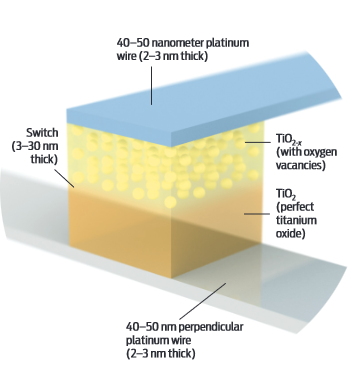
\includegraphics[width=0.6\textwidth]{mem1.png}
		\caption{Costruccion del memristor de HP. Referencia: \cite{williams}}
		\label{fig:mem1}
	\end{figure}
	
	El oxido de titanio tiene una serie de caracteristicas que lo hacen un material muy interesante en esta aplicacion:
	\begin{enumerate}
		\item Resistencia variable: La resistencia electrica del oxido de titanio puede cambiar en repuesta de la aplicacion de una corriente o un campo electrico. Lo cual nos permite no tan solo guardar 1 o 0 si no un rango de valores dentro de unos limites de operacion.
		\item No volatilidad: El óxido de titanio puede mantener su estado de resistencia incluso cuando se retira la corriente eléctrica que lo atraviesa. Esto significa que puede retener información y mantener su estado de resistencia sin requerir energía continua.
		\item Cambios rápidos de resistencia:  Esta propiedad permite operaciones de escritura y lectura rápidas en el memristor, lo que es crucial para su uso en aplicaciones de almacenamiento y procesamiento de datos.
		\item Baja potencia y tamaño compacto
	\end{enumerate}
	\newpage
	
	La formula que se propone en \cite{HP} para modelar el comportamiento de este dispositivo es:
	
	\begin{equation}
		v(t)\,=\,\left(R_{ON}\,\frac{w(t)}{D}+R_{OFF}\left(1-\frac{w(t)}{D}\right)\right)i(t)
		\label{eq:hp1}
	\end{equation}
	
	\begin{equation}
		\frac{dw(t)}{dt}\,=\,\mu_V\,\frac{R_{ON}}{D}\,q(t)
		\label{eq:hp2}
	\end{equation}\smallskip
	
	Integrando la ecuación \eref{eq:hp2} e insertandola en \eref{eq:hp1} teniendo en cuenta que el valor de resistencia  $R_{ON} \ll R_{OFF}$: 
	
	\begin{equation}
		w(t)\,=\,\mu_V\,\frac{R_{ON}}{D}\,i(t)
		\label{eq:hp3}
	\end{equation}\smallskip
	\begin{equation}
		M(q)\,=\,R_{OFF}\,\left(1-\,\frac{\mu_V\,R_{ON}}{D^2}\,q(t)\right)
		\label{eq:hp4}
	\end{equation}\smallskip
	
	\begin{figure}[h]
		\centering
		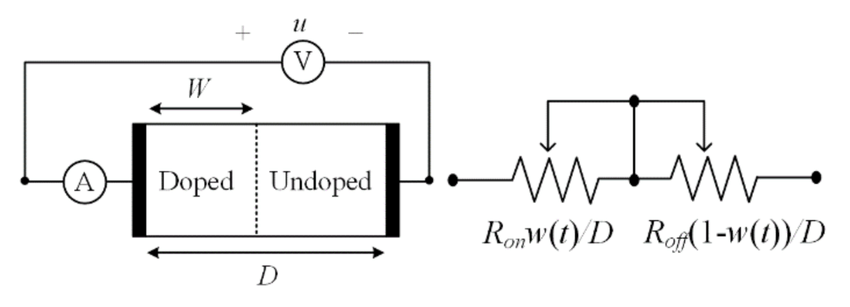
\includegraphics[width=1\textwidth]{schmem.png}
		\caption{Esquema del memristor de HP. Referencia: \cite{2021}}
		\label{fig:2021}
	\end{figure}\smallskip
	
	Los parámetros que aparecen en las ecuaciones anteriores y que describen el funcionamiento del componente son:
	
	\begin{enumerate}
		\item $R_{ON}$: Resistencia en el estado ON, valor mínimo. Es constante.
		\item $R_{OFF}$: Resistencia en el estado OFF, valor máximo. Es constante.
		\item $\mu_V$: Mobilidad iónica de arrastre promedio. Es constante.
		\item $w$: Ancho de la zona dopada, no es constante, depende de la excitación.
		\item $D$: Ancho total de la lamina de oxido de titanio. Es constante.
	\end{enumerate}
	\newpage
	
	El funcionamiento es el siguiente, entre los dos electrodos de platino tenemos una capa de dióxido de titanio puro $TiO_2$ que actúa como dieléctrico y otra de dióxido de titanio con vacantes de oxígeno $TiO_{2-x}$ que actúa como conductor ya que en estas vacantes están cargadas positivamente (ver \fref{fig:mem1}), ya que al faltar atomos de oxígeno se están perdiendo también sus electrones de valencia asociados, generando así que el compuesto necesite atraer electrones a dichas vacantes para así mantenerse electricamente estable.Cuando un voltaje positivo se aplica al electrodo superior las vacantes de oxígeno de la zona dopada se repelen y viajan hacia la zona de oxido de titanio puro, haciendo asi que aumente la conductividad hasta que se alcance el valor de $R_{ON}$. Si por el contrario el voltaje aplicado es negativo, las vacantes de oxígeno viajan hacia el elctrodo superior, reduciendo la conductividad hasta $R_{OFF}$.
	
	\begin{figure}[h]
		\centering
		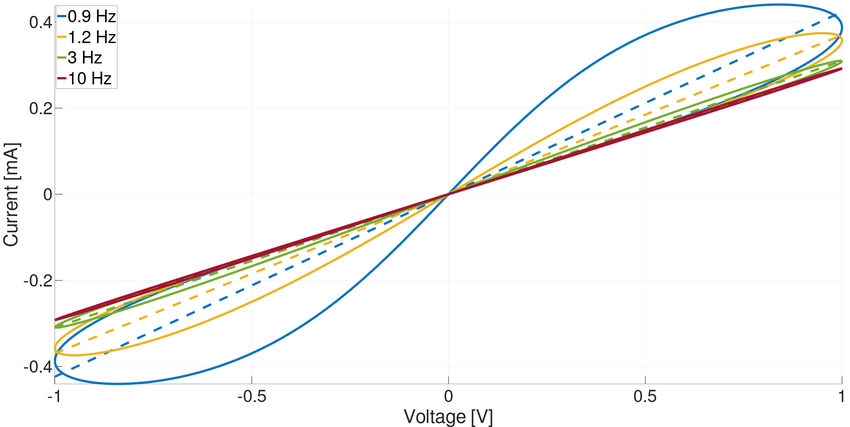
\includegraphics[width=0.8\textwidth]{iv_chua.png}
		\caption{Gráfica Tensión-Intensidad del Memristor de Chua ideal para una señal de entrada senoidal con varias frecuencias. Como se puede ver conforme aumenta la frecuencia la gráfica se parece más a la de una resistencia tradicional. \\ Referencia: \cite{outsiders}}
		\label{fig:iv_chua}
	\end{figure}\smallskip
	
		\begin{figure}[h]
		\centering
		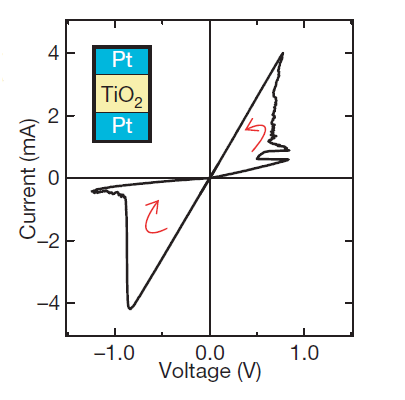
\includegraphics[width=0.5\textwidth]{iv_hp.png}
		\caption{Gráfica Tensión-Intensidad del Memristor de HP. Referencia: \cite{HP}}
		\label{fig:iv_hp}
	\end{figure}\smallskip
	
	\newpage
	
	\section{Variables de estado}
	En este trabajo hemos hecho un análisis matemático de la bifurcación del circuito oscilador haciendo uso de técnicas de análisis de reciente estudio, pero primero hay que presentar el circuito y transformar sus ecuaciones eléctricas hasta llegar a una forma matemática con la que poder trabajar, por ello empecemos analizando el circuito.
	
	\begin{figure}[h]
		\centering
		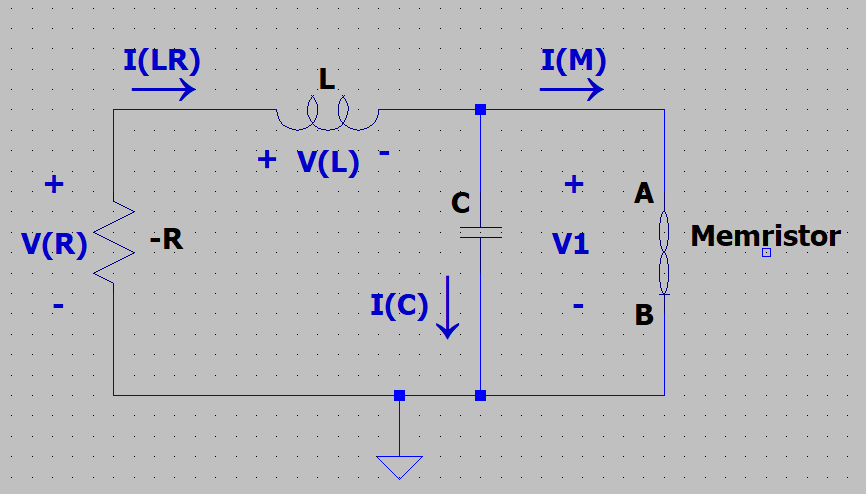
\includegraphics[width=0.8\textwidth]{circuito.png}
		\caption{Parámetros del circuito}
		\label{fig:circuito}
	\end{figure}\smallskip
	
	Aplicanco las leyes de Kirchoff a nuestro circuito, \fref{fig:circuito}, se puede ver que:
	
	\begin{equation}
		i_{LR}\,=\,i_M+i_C
		\label{eq:kir1}
	\end{equation}
	\begin{equation}
		v_R\,=\,v_L+v_1
		\label{eq:kir2}
	\end{equation}
	
	Reordenando las anteriores ecuaciones:
	
	\begin{equation}
		i_C\,=\,i_{LR}-i_M
		\label{eq:kir11}
	\end{equation}
	\begin{equation}
		v_L\,=\,v_R-v_1
		\label{eq:kir22}
	\end{equation}
	
	Recordando la relación entre la carga y el flujo con la intensidad y la tensión de las ecuaciones \eref{eq:dvdi}, la ecuación del memristor controlado por flujo \eref{eq:fc} y aplicándolo a \eref{eq:kir11} y \eref{eq:kir22} obtenemos:
	
	
	\begin{eqnarray}
		C\,\frac{dv_1}{dt}\,&=&\,i_{LR}-W(\varphi)\,v_1 \label{eq:kir111} \\ [2mm]
		L\,\frac{di_{LR}}{dt}\,&=&\,R\,i_{LR}-v_1 \label{eq:kir222} \\ [2mm]
		\frac{d\varphi}{dt}\,&=&\,v_1 \label{eq:kir333}
	\end{eqnarray}\smallskip
	
	Como se pueden ver las variables de estado elegidas son la intensidad en la resistencia y la bobina \bm{$i_{LR}$}, la tensión en el condensador y el memristor \bm{$v_1$} y el flujo en el memristor \bm{$\varphi$}
	\newpage
	Reordenando las ecuaciones anteriores \eref{eq:kir111}, \eref{eq:kir222} y \eref{eq:kir333} tenemos:
	
	\begin{eqnarray}
		\frac{dv_1}{dt}\,&=&\,\frac{i_{LR}}{C}-W(\varphi)\,\frac{v_1}{C} \label{eq:sis1} \\ [2mm]
		\frac{di_{LR}}{dt}\,&=&\,\frac{R}{L}\,i_{LR}-\frac{v_1}{L} \label{eq:sis2} \\ [2mm]
		\frac{d\varphi}{dt}\,&=&\,v_1 \label{eq:sis3}
	\end{eqnarray}\smallskip
	
	Haciendo algunos cambios a las tres anteriores ecuaciones para luego poder trabajar con las ecuaciones obtenemos el siguiente sistema:
    
	\begin{equation}
		\label{eq:sistema}
		\scalebox{1.2}{$\displaystyle
			\left\{
			\begin{aligned}
				\frac{dx}{dt} &= \alpha (y - W(z)x) \\
				\frac{dy}{dt} &= -\xi x + \beta y \\
				\frac{dz}{dt} &= x
			\end{aligned}
			\right.
			$}
	\end{equation}\smallskip
	Donde tenemos:
	\begin{equation*}
		x\,=\,v_1 \qquad y\,=\,i_{LR} \qquad z\,=\,\varphi \qquad \& \qquad \alpha\,=\,\frac{1}{C} \qquad \beta\,=\,\frac{R}{L} \qquad \xi\,=\,\frac{1}{L}
	\end{equation*}
	
	Pero del sistema \eref{eq:sistema} aun tenemos que definir $W(z)$. En \cite{chuaoscillator2008} se asume que el comportamiento del memristor se puede aproximar por una ecuacion linear a trozos monótonamente creciente:
	
	\begin{equation}
		q(\varphi)\,=\,b\varphi+0.5(a-b)(|\varphi+1|-|\varphi-1|)
		\label{eq:qf}
	\end{equation}
    \begin{center}
    	$\forall\quad a,b,c,d> 0$
    \end{center}
    
    Escribiendo \eref{eq:qf} con la variable \bm{$z$} y derivandola (recordando la ecuación \eref{eq:myw}) para obtener $W(z)$:
    
    \begin{equation}
    	q(z)\,=\,bz+0.5(a-b)(|z+1|-|z-1|)
    	\label{eq:qfz}
    \end{equation}
    
    \begin{equation}
    	W(z)\,=\,\frac{dq(z)}{dz}\,=\,
    		\label{eq:wz}
    		\scalebox{1}{$\displaystyle
    			\left\{
    			\begin{aligned}
    				a, \quad   |z| < 1\\
    				b, \quad   |z| > 1
    			\end{aligned}
    			\right.
    			$}
    \end{equation}
    
	Ya tenemos las ecuaciones necesarias para empezar el análisis pero primero veremos en los siguientes capitulos que técnicas estaremos usando para ello.
	\newpage
	\section{Superficies invariantes}
	esto es texto de la siguiente hoja
	
	\chapter{Sistemas Lineales a Trozos Bizonales}
	Contenido del capítulo 3.
	\newpage
	\section{Sistemas lineales planos}
	esto es texto de la siguiente hoja
	\newpage
	\section{Sistemas lineales a trozos bizonales}
	esto es texto de la siguiente hoja
	
	\chapter{Semiaplicaciones de Poincaré}
	Contenido del capítulo 4.
	\newpage
	esto es texto de la siguiente hoja
	
	\chapter{Bifurcación Foco-Centro-Ciclo Límite}
	Contenido del capítulo 5.
	\newpage
	esto es texto de la siguiente hoja
	
	\chapter{Oscilación Peródica en el circuito}
	Contenido del capítulo 6.
	\newpage
	esto es texto de la siguiente hoja
	
	\chapter{TÍTULO CAPÍTULO 7}
	Contenido del capítulo 7.
	\newpage
	esto es texto de la siguiente hoja
	
	\chapter{TÍTULO CAPÍTULO 8}
	Contenido del capítulo 8.
	\newpage
	esto es texto de la siguiente hoja
	
	\chapter*{Conclusiones}
	Contenido del capítulo de conclusiones.
	\newpage
	
	
	\begin{thebibliography}{99}
		\bibitem{chuamissing1971} CHUA, L. O. Memristor – The missing circuit element. IEEE
		Transactions on Circuit Theory, 1971, vol. CT-18, no. 5, p. 507 to
		519. DOI: 10.1109/TCT.1971.1083337.
		
		\bibitem{chuaoscillator2008} Itoh, Makoto \& Chua, Leon. (2008). Memristor oscillators. I. J. Bifurcation and Chaos. 18. 3183-3206. 10.1142/S0218127408022354. 
		
		\bibitem{HP} Strukov DB, Snider GS, Stewart DR, Williams RS. The missing memristor found. Nature. 2008 May 1;453(7191):80-3. doi: 10.1038/nature06932. Erratum in: Nature. 2009 Jun 25;459(7250):1154. PMID: 18451858.
		
		\bibitem{williams} R. S. Williams, "How We Found The Missing Memristor," in IEEE Spectrum, vol. 45, no. 12, pp. 28-35, Dec. 2008, doi: 10.1109/MSPEC.2008.4687366.
		
		\bibitem{2021} Xiaoyue, Ji \& Dong, Zhekang \& Zhou, Guangdong \& Lai, Chun Sing \& Yan, Yunfeng \& Qi, Donglian. (2021). Memristive System Based Image Processing Technology: A Review and Perspective. Electronics. 10. 3176. 10.3390/electronics10243176. 
		
		\bibitem{outsiders} Caravelli, F. \& Carbajal, Juan. (2018). Memristors for the Curious Outsiders. 10.31224/osf.io/c4qr9. 
		
	\end{thebibliography}
	
	\newpage
	
	\begin{comment}
	\chapter{Introducción}
	\begin{equation}
		\label{EcuLambda}
		y^2=3
	\end{equation}
	hola mundo prueba script prueba branch de funcion $f$ \eqref{EcuLambda} en $[2\pi]$
	\newpage
	holaaa
	\newpage
	asldkakdlkad prueba python para commit cambio
	\newpage
	\section{introa}
	holaaa
	\newpage
	\subsection{introb}
	segundo cambio tercera prueba python siguiente prueba para ver fuente
	\end{comment}
\end{document}
